% !TEX root = ../main.tex
% !TEX spellcheck = en_GB

\chapter{Requirements}

In this chapter the requirements for the system will be described.
A single use case has been defined, which describes the functionality and the actor's interaction with the system \systemName.
These use case establish the foundation of the requirements specification.

\begin{figure}[H]
	\centering
	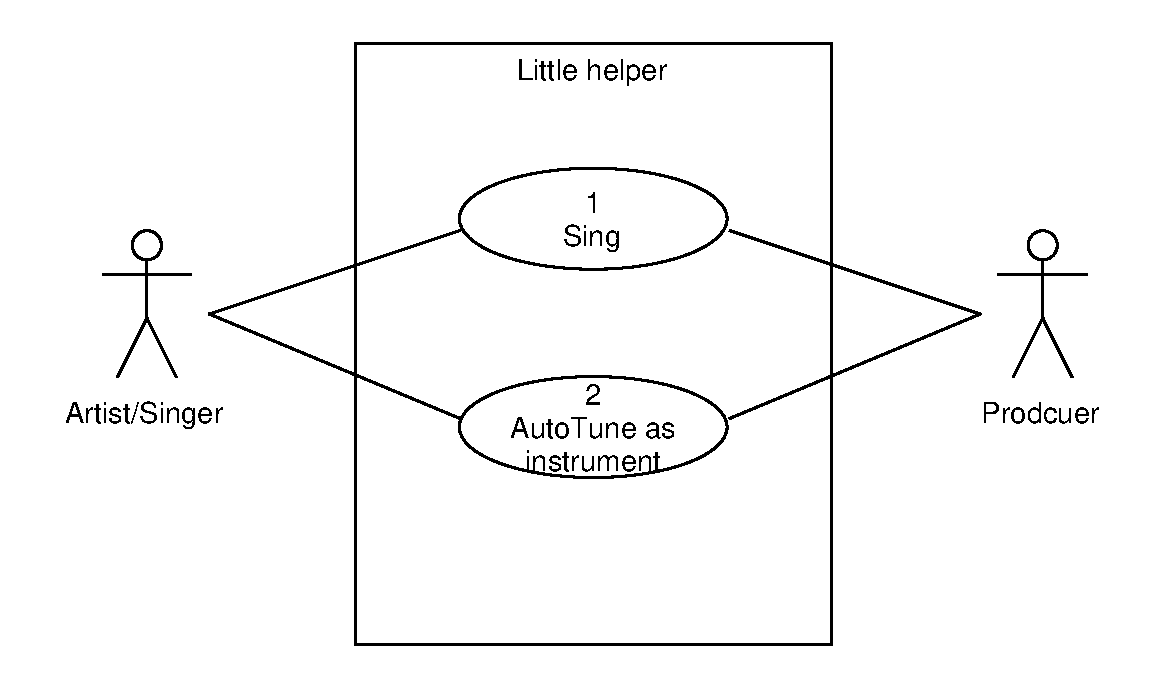
\includegraphics[width=0.7\linewidth]{Design/UseCaseDiagram.pdf}
	\caption{Use Case diagram.}
	\label{fig:UCDiagram}
\end{figure}

\section{Actor descriptions}

\begin{table}[H]
	\centering
	\begin{tabularx}{\textwidth}{p{0.2\textwidth} X}
		\toprule
		\textbf{Name of actor} & Artist \\
		\textbf{Type} & Primary \\
		\textbf{Description} & Is a live performer.
		The goal for the Artist can be either to be corrected into perfect pitch (e.g. from \SI{443}{\hertz} to \SI{440}{\hertz}), or to create the robotic sound often associated with auto tune (e.g. Cher - Believe). \\
		\bottomrule
	\end{tabularx}
	\caption{Actor description of Artist.}
	\label{tab:actorArtist}
\end{table}

\begin{table}[H]
	\centering
	\begin{tabularx}{\textwidth}{p{0.2\textwidth} X}
		\toprule
		\textbf{Name of actor} & Producer \\
		\textbf{Type} & Primary \\
		\textbf{Description} & Decides how the sounds are during recordings. The producer needs to be able to change the amount of auto tuning used during the recording, to find the right balance. \\
		\bottomrule
	\end{tabularx}
	\caption{Actor description of Producer.}
	\label{tab:actorProducer}
\end{table}

\begin{table}[H]
	\centering
	\begin{tabularx}{\textwidth}{p{0.2\textwidth} X}
		\toprule
		\textbf{Name of actor} & Audience \\
		\textbf{Type} & Secondary \\
		\textbf{Description} & The recipient of the live performance or studio recording. Is interested in hearing the music as the Artist/Producer intended it to be heard. \\
		\bottomrule
	\end{tabularx}
	\caption{Actor description of Audience.}
	\label{tab:actorAudience}
\end{table}

\section{Use Cases}
\label{rap:UC}
\Cref{fig:UCDiagram} shows the defined use cases and the different actors involved in each of them.

\subsection{Use Case 1 - Pitch correction}

\begin{table}[H]
	\centering
	\begin{tabularx}{\textwidth}{p{0.3\textwidth} X}
		\toprule
		\textbf{Name} & Pitch correction \\
		\midrule
		\textbf{Goal} & To move an off tune sound onto a piano scale tune. \\
		\midrule
		\textbf{Initiation} & Singing commences.\\
		\midrule
		\textbf{Actors and Stakeholders} & Artist, Producer and Audience. \\
		\midrule
		\textbf{Precondition} & Resolution and scale is set. \\
		\midrule
		\textbf{Post-condition} & Output sound is moved to the nearest on-pitch frequency, determined by the resolution and scale. \\
		\midrule
		\textbf{Main scenario} & 
		\begin{enumerate}[noitemsep, topsep=0pt]
			\item Artist starts singing off pitch.
			\item Artist/Producer engages Pitch correction.
			\item[\textbf{EXT1}] Artist/Producer is not satisfied with set scale or resolution.
			\item Output sound is on pitch according to the set resolution.
		\end{enumerate}
		\\
		\midrule
		\textbf{Extension} & 
		\textbf{EXT1}
		\begin{enumerate}[noitemsep, topsep=0pt]
			\item Sound is not as Artist/Producer wants it.
			\item Artist/Producer changes resolution or scale.
			\item Output sound is on pitch according to the set resolution.
		\end{enumerate}
		\\
		\bottomrule
	\end{tabularx}
\end{table}

\section{Functional Requirements}
A MoSCoW based on the above use case is presented below to account for the functional requirements.

\begin{itemize}
	\item[MUST] ~
	\begin{itemize}
		\item \systemName must shift the primary frequency of the input signal to the nearest step on the desired scale.
		\item \systemName must do the processing quickly, so there is no audible delay in the sound.
		\item \systemName must do the processing so there is no noticeable noise when the input frequency changes.
	\end{itemize}
	\item[SHOULD] ~
	\begin{itemize}
		\item The user should be able to change how 'effective/strong' the auto tune is by pressing buttons on the system.
		\item The user should be able to turn auto tuner on/off by pressing a button.
		\item Little helper should have a LED indicating if it is on or off.
		\item Little helper should have 4 LED's indicating which level the auto tuner is on where 0 LED's on is low. and 4 LED's on is high.
	\end{itemize}
	\item[COULD] ~
	\begin{itemize}
		\item \systemName could be configured by a GUI, so the user can change all the different parameters, such as scale, force and speed.
		\item \systemName could take noisy environment into account, when finding the primary frequency.
	\end{itemize}
	\item[WON'T] ~
	\begin{itemize}
		\item \systemName won't make you sing like Freddie Mercury.
	\end{itemize}
\end{itemize}

\section{Non-functional Requirements}
\label{sec:nonfunc}
\begin{itemize}
	\item[R1] \systemName must process audio signals in the C-major scale (\SIrange{261.626}{493.883}{\hertz}).
	\item[R2] \systemName must correct the audio signal to the nearest step on the scale \SI{\pm 2.5}{\hertz}.
	\item[R3] \systemName latency should be less than \SI{50}{\milli\second}.
	\item[R4] The filter algorithm must be realized using build-in fixed point fractional types (fract16, fract32).
	\item[R5] \systemName should fill less than \SI{16}{\kilo\byte}.
	\item[R6] The filter should be optimized in speed performance for the B533.
	\item[R7] The filter should have a maximum DSP load of \SI{95}{\percent}.
\end{itemize}

\section{Derived Requirements}
\begin{itemize}
	\item[DR1] \systemName must sample with a samle rate of \SI{48}{\kilo\hertz}.
	Derived from R1, where $f_{max}=\SI{1046.5}{\hertz}$ then minimum sampling frequency must be $fs_{min} = f_{max}\cdot 2 = \SI{2093}{\hertz}$.
	\item[DR2] The filter latency must be delayed by a maximum of \num{2000} samples.
	Derived from R3 where the latency is less than \SI{50}{\milli\second}, $f_s = \SI{48}{\kilo\hertz}$, $t_d = \SI{41}{\milli\second}$.
	\item[DR3] The filter must use a maximum of \num{11875} cycles of DSP processing per sample. Derived from R6, R7 and DR1.
	$\frac{\SI{600}{\mega\hertz}}{\SI{48}{\kilo\hertz}}\cdot\SI{95}{\percent} = \num{11875}$.
\end{itemize}

